\documentclass[dvips,12pt]{article}

\usepackage[pdftex]{graphicx}
\usepackage{helvet}
\usepackage[ngerman, english]{babel} 
\usepackage[a4paper, left=3cm, right=3cm, top=1.3cm]{geometry}
\usepackage{url}
\usepackage{fancyhdr}
\usepackage{booktabs}
\usepackage{titlesec}
\usepackage{tabularx}
\usepackage{verbatim}

\renewcommand{\familydefault}{\sfdefault}
\renewcommand{\baselinestretch}{1.4}\normalsize
\setlength{\parskip}{11px}
\setlength{\parindent}{0pt}
\setlength{\oddsidemargin}{0.25in}
\setlength{\textwidth}{6.5in}
\setlength{\topmargin}{0in}
\setlength{\textheight}{8.5in}

\begin{document}

\title{
\begin{center}
\resizebox{6in}{!}{\includegraphics*{../epic.png}}
\end{center}
Proposal
}

\author{Jan Kerkenhoff, Miguel Gonzalez}
\date{\today}

\maketitle

\section{Motivation}

This document describes, how we want to plan our project, which features should be included and what we want to improve. The first attempt was to improve the existing version of \textbf{Extreme text adventure}. After we read the minimalistic documentation it is now our aim not only to improve the software - we want to introduce a more generic way of making text adventures.\\

We have finally decided to create a tool to generate text adventures by taking a XML file into account. In the following we explain, how we want to achieve the goal of a full-working game generator within 7 weeks of work.

\section{Introduction}

Text adventures can be the most powerful game experience on earth, because you're able to create all graphics, events and sounds in your head. You type in commands and the game reacts. Sometimes events happen, a troll may arrack you suddenly or you find mighty items in order to improve your hero. Therefore we can derrive the following entities in each game, which can be defined by the user of your software in XML:

\begin{itemize}
	\item{\textbf{Room}: a player can only be in one room at times. The room can be called whatever the designer decides. (for instance, desert, forest, dungeon)}
	\item{\textbf{Player}: the player in the world}
	\item{\textbf{Item}: an item which can be collected, used or equiped by the player.}
	\item{\textbf{Creature}: A creature can be allied, neutral or be your enemy. Additionally, creatures can hold items. Creatures may drop these items if they get killed.}
	\item{\textbf{Door}: A door simply is a connection between two rooms. Each door can have a guard which avoids passing.}
\end{itemize}

Our software should provide an interface for the user to create the content from above in XML, by defining first all existing entities and then creating the world (rooms and fill them with content).

\section{World design}

As mentioned before, the world is devided into rooms. These rooms can be visited by the player. For some rooms he may need permission. In that case, he has to fit some requirements. These requirements (or guards) can be set in XML as well. Let us have a look at a simple world:

\begin{figure}[hb]
  \centering
  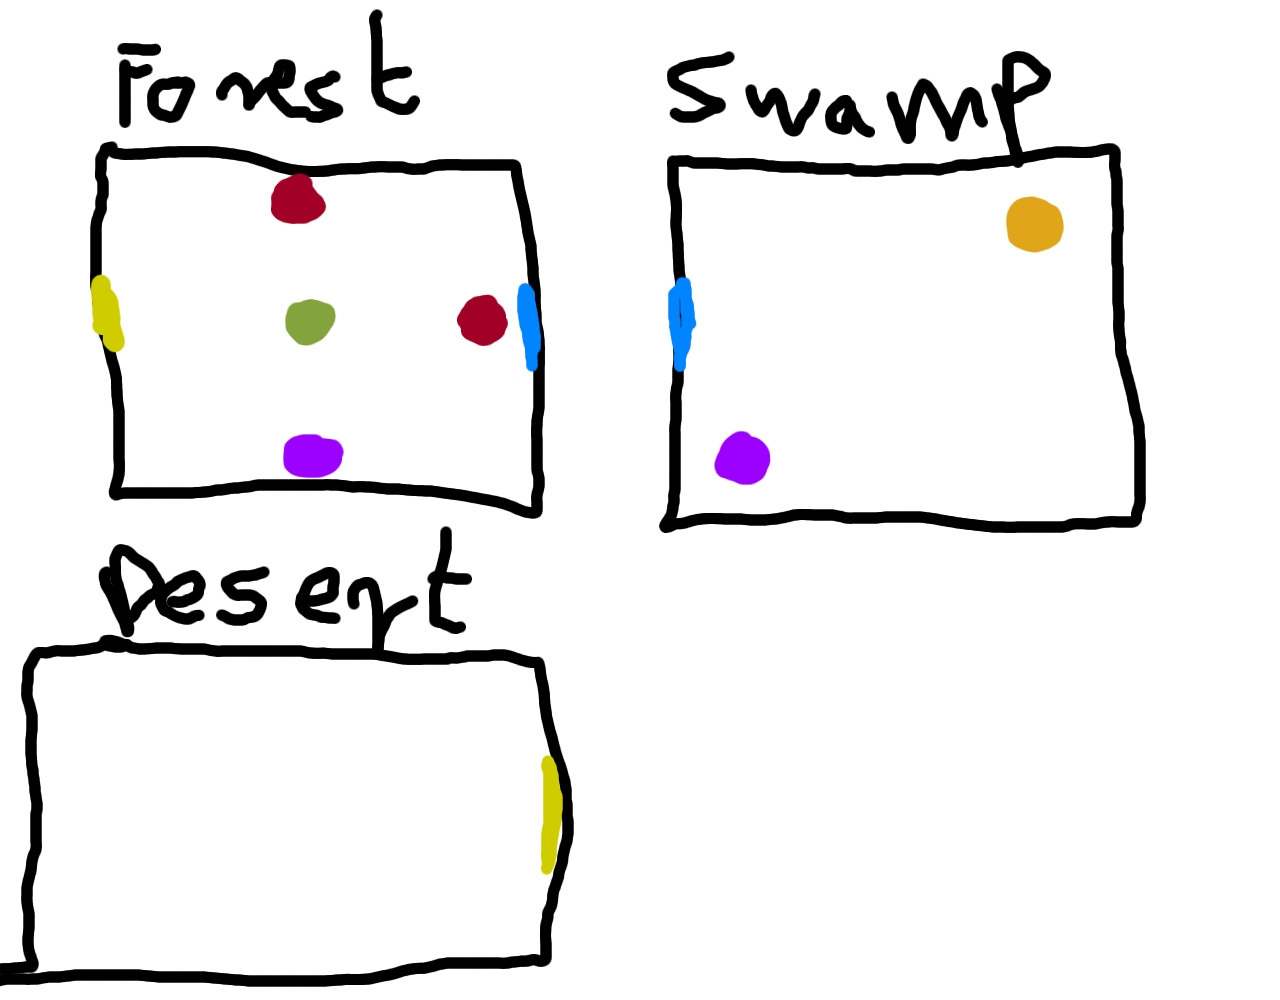
\includegraphics[width=4in]{../demo/demo.jpg}
  \caption{Each room is divided into 9 parts.}
\end{figure}

We want to create a simple world design where each room can have 9 parts. On each part can only be one game object at one time. It's also possible to move the player in a room or to pass doors due to enter other rooms. It is also possible to put game objects in each room. As you can see in the image, the green point is the player, the red ones are enemies, the yellow point is a neutral creature and the violet points are items, laying on the ground.

\subsection{Transition into XML}

To create such a world from above, we want to make it possible to create XML synthax just like in the appended XML file (see page \ref{App:xml}).

\section{Java API}

We also want to provide a simple Java API which can be used in order to create own text adventures. Let us imagine, we have created such a content file, called \emph{my-game.xml}. To create a text adventure by using our library, the user may write something like this:

\begin{verbatim}
TextAdventure adventure = new TextAdventure(new XMLSource("my-game.xml"));

adventure.addListener(new AdventureListener() {

    @Override
    public void onAction(AdventureEvent event) {
       // Do something with the output
    }
});

// Add command
adventure.command("go west");
\end{verbatim}

It is possible to enter commands to the adventure object or to fetch a response by just adding listeners. We used the listener approach because it is very easy to use our library in combination with a GUI.


\section{Commands}

Also a very important part are commands. Commands are the only way in a text adventure to interact with the game. We decided to create basic commands to interact with the current game world:

\begin{itemize}
	\item{\textbf{go} [\emph{west} | \emph{east} | \emph{north} | \emph{south}]}
	\item{\textbf{attack} \emph{creature name}}
	\item{\textbf{take} [\emph{item name} | \emph{all}]}
	\item{\textbf{drop} \emph{item name} | \emph{all}]}
	\item{\textbf{use} \emph{item name}}
	\item{\textbf{open} [\emph{\emph{door name} | \emph{chest name}}]}
\end{itemize}

The player can use these commands any time. If an action doesn't work (for instance, the item doesn't exit or there is nothing to attack), a message will be generated.

\section{Conclusion}

We want to create a proper way of making text adventures more easily. This project may improve our development and API design skills as well as pushing our XML knowledge.

\section{Appendix}

\label{App:xml}

\subsection{Sample XML file}


XML file to display the world from \emph{Figure 1}.
\verbatiminput{../demo/demo.xml}

\subsection{API design}
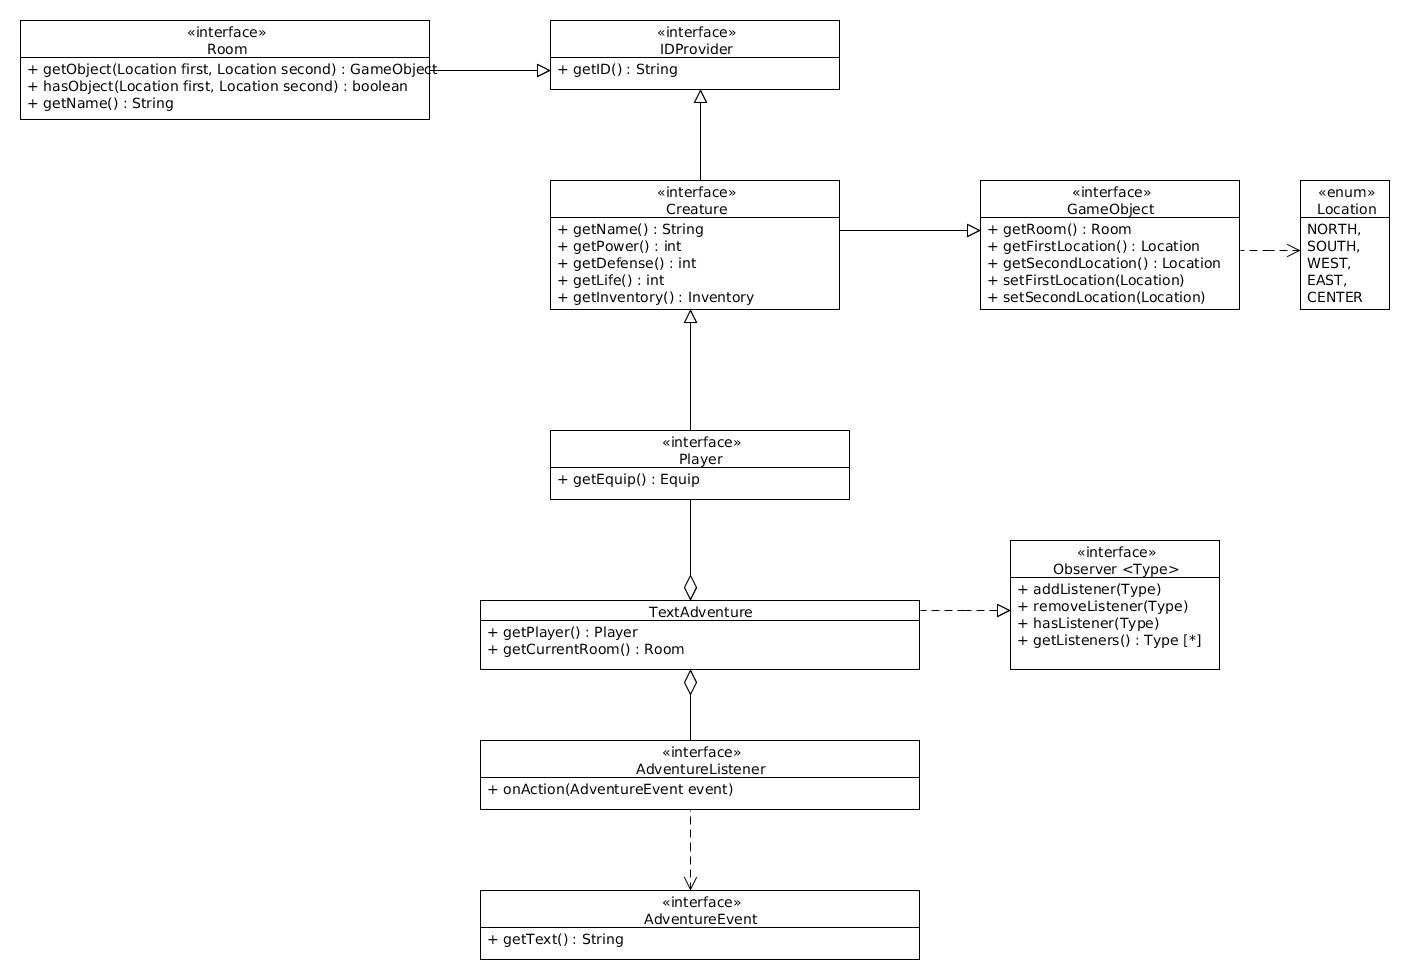
\includegraphics[width=6.5in]{assets/class-diagram.png}

\end{document}

